\documentclass[12pt,a4paper,landscape]{article}
\usepackage{geometry}
\geometry{left=2.5cm,right=2.5cm,top=2.5cm,bottom=2.5cm}

\usepackage[utf8]{inputenc}
\usepackage{listings}
\usepackage{CJK}
\usepackage{xcolor}
\usepackage{graphicx}


\begin{document}
\begin{CJK}{UTF8}{gbsn}
\title{GoAgent网站证书不受信任解决方法(windows + Chrome)}
\author{ismdeep}
\date{2013-8-5 15:37:06}


\maketitle

%设置listings
\lstset{numbers=left,
numberstyle=\tiny,
keywordstyle=\color{blue!100}, commentstyle=\color{red!50!green!50!blue!50},
frame=single,tabsize=4,showtabs=false,extendedchars=false,
rulesepcolor=\color{red!20!green!20!blue!20}
}



%正文开始
\newpage

这段时间以及之前的一段时间内,用GoAgent翻墙上登自己的Facebook账号就出现如下情况。


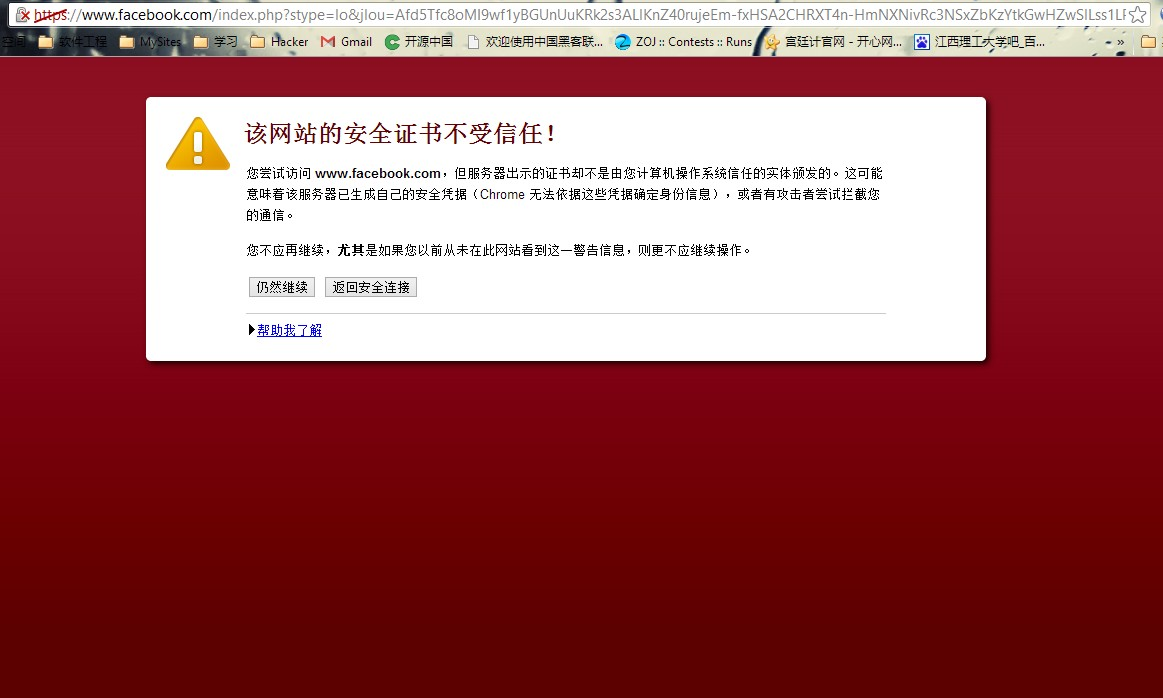
\includegraphics[scale=0.55]{pic/001.jpg}

\newpage

到处找了下,原来是需要安装一个证书,而证书就在GoAgent里面有的,在local文件夹里面


\includegraphics[scale=1.5]{pic/002.jpg}


\newpage

这个就很好解决了。。双击CA.crt安装证书即可。


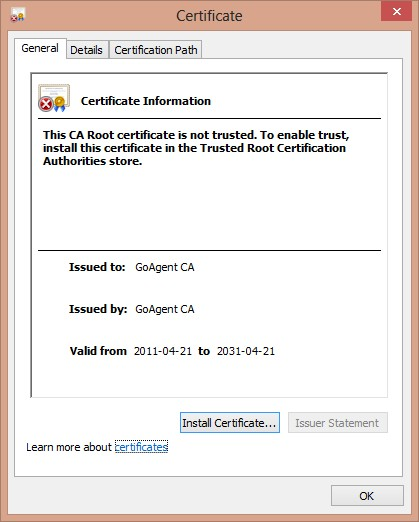
\includegraphics[scale=1]{pic/003.jpg}


\includegraphics[scale=1]{pic/004.jpg}


\includegraphics[scale=1]{pic/005-1.jpg}

\includegraphics[scale=1]{pic/005-2.jpg}

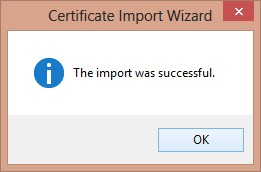
\includegraphics[scale=1]{pic/006.jpg}



\newpage

导入证书之后,还是会显示下面这样的。

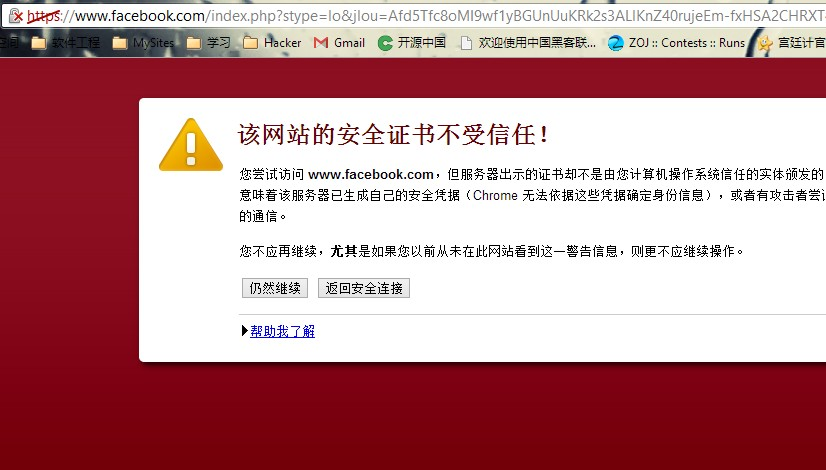
\includegraphics[scale=1]{pic/007.jpg}

\newpage

这里需要重启一下GoAgent,好吧,,走,重启去。。。

重启之后。最好重启一下浏览器。。

然后就可以了。。。不会有那种困扰了。。

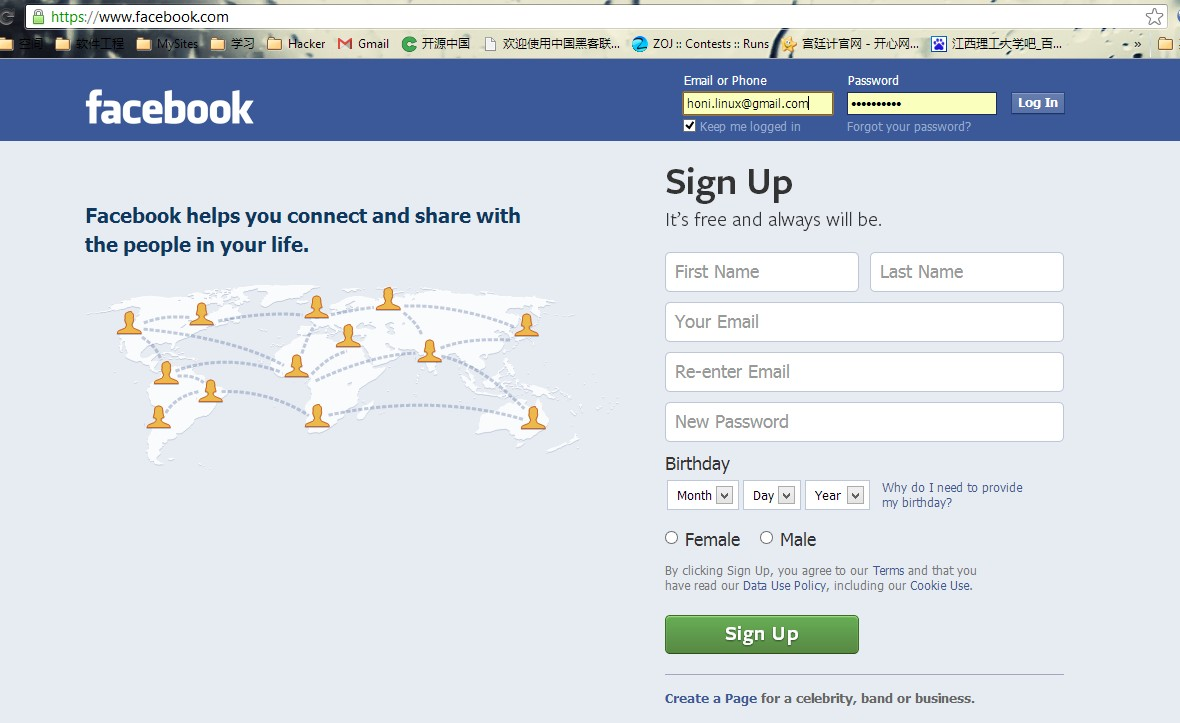
\includegraphics[scale=0.75]{pic/008.jpg}


\newpage
\Large{更多教程请访问。

$http://git.oschina.net/ismdeep/public\_documents$

或者发送邮件到: izumu@ism.name 或 honi.linux@gmail.com 共同交流

}

\end{CJK}
\end{document}


